\subsubsection{Lunar Farside Location}
The lunar farside is a unique location in the solar system in that it is the only area that never faces the Earth due to tidal locking.  This means that it is always blocked from terrestial and near-terrestrial radio frequency transmissions.  This importance was recognized in the 1970s when the International Telecommunication Union (ITU\footnote{The ITU is the international organization that handles electromagnetic emission across national boundaries.} defined the Shielded Zone of the Moon (SZM) as “compris[ing] the area of the Moon’s surface and an adjacent volume of space which are shielded from emissions originating within a distance of 100,000 km from the center of the Earth” \citep{itu_rr_2024}.  It is this essential radio quietness that LFT3 wishes to exploit.

The landing site coordinates of 23.78930°S, 182.13737°E are well within the SZM and are additionally near the LuSEE-Night landing location.  In the Equatorial Farside region, lunar days and lunar nights each last approximately 14 Earth days. This results in survival temperatures ranging from 213 to 348 K.

    
\begin{figure}
	\centering
	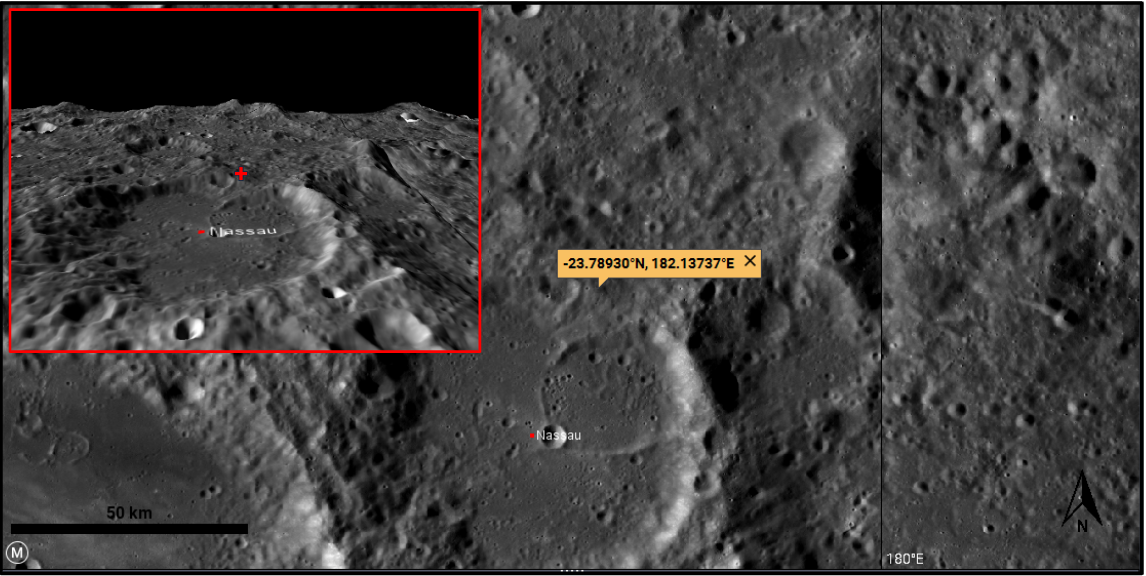
\includegraphics[width=\linewidth]{figures/Landing site overview.PNG}
	\caption{LFT3 Farside Landing Site - Micro View JMARS}
\end{figure}


\subsection{Site Regolith Conditions}
\textit{Study needed}
Regolith characteristics of the site are well known, to include regolith of no larger than X? size. Allowing proper landing conditions to exist for touchdown and operations. Not obstructing landing operations in depth, to include power down and gimbling. Upon initial touchdown the lander will experience expected position settling onto the regolith surface. Regolith characteristics will impact the final field of regard. Mission requirement of measuring the lander tilt will be taken once in position, on the lunar surface, for calibrated data.